\chapter{Servidor de mapas dinámico}
\label{cap:sevidordemapasdinamico}


En este capítulo se explica la construcción y el funcionamiento del servidor de mapas dinámico. En primer lugar se explica que es, para que se utiliza y como se construye un \textit{costmap}. En segundo lugar se explica como se construyen los mapas que componen el algoritmo y por último se explica como se combinan estos mapas para generar el mapa usado en la navegación.

\section{Costmap\_2D}
\label{sec:costmap2d}
Un \textit{costmap} es una estructura de datos ofrecida por ROS y compuesta por un grid de ocupación y los metadatos de este grid. Cada celda del grid toma valores entre 0 y 255, donde 0 corresponde a una celda vacía, los valores entre 1 y 254 representan la probabilidad de que una celda está ocupada y el valor 255 se reserva para el desconocimiento. Cada valor se asocia con un nivel de gris, como se puede ver en la imagen.
\begin{figure} [hbtp]
  \begin{center}
    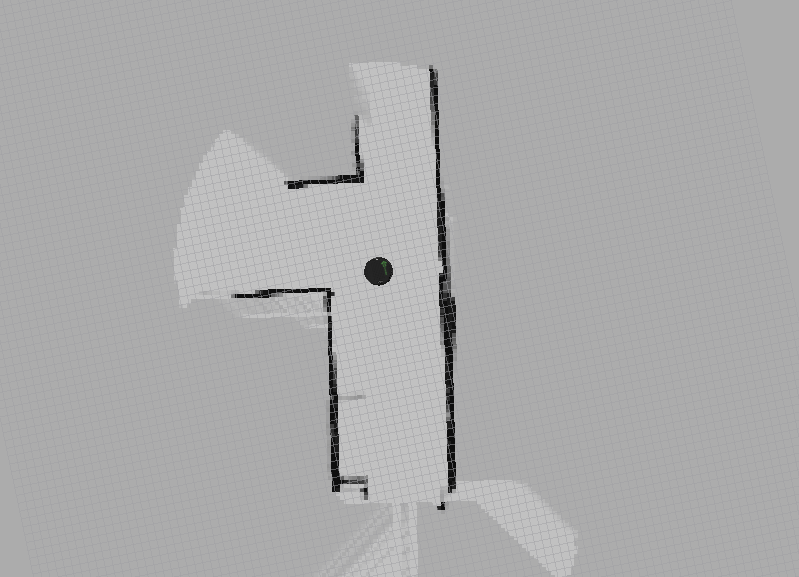
\includegraphics[width=7.5cm]{img/cap4/costmap-ejemplo}
  \end{center}
  \caption{Ejemplo visual de un costmap.}
  \label{fig:costmap-ejemplo}
\end{figure}\

Para poder representar la ocupación de un objeto en un \textit{costmap} es necesario hacer uso de las transformadas entre frames que nos ofrece ROS.

\subsubsection{tf}
\label{subsubsec:tf}
Cualquier robot está compuesto por multitud de piezas móviles, como puede ser la propia base del robot o la pinza de un brazo robótico. Cada una de estas piezas se pueden representar con un \textit{frame}. Ademas existen también otros \textit{frames} que pueden interesarnos, como puede ser el \textit{frame} de world o el \textit{frame} de map.
\begin{figure} [hbtp]
  \begin{center}
    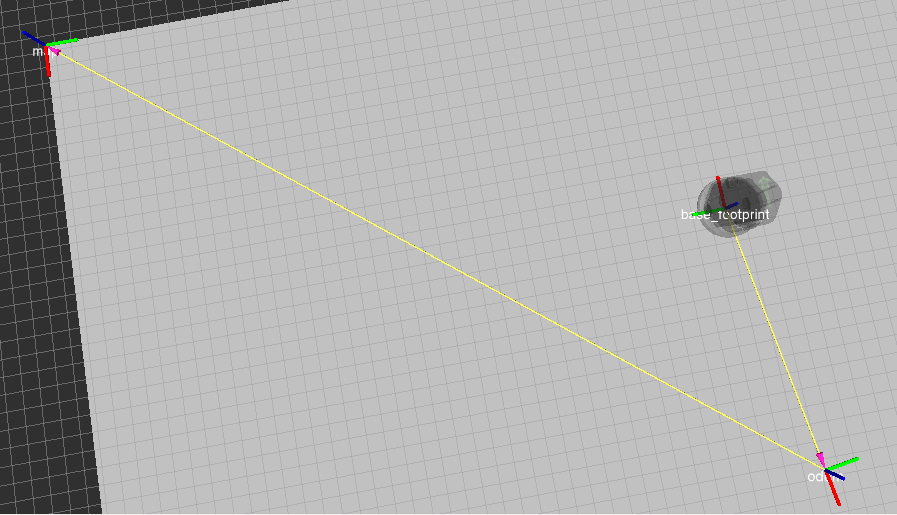
\includegraphics[width=12cm]{img/cap4/frames}
  \end{center}
  \caption{A la izquierda el frame map y a la derecha los frames de odom y base\_footprint}
  \label{fig:frames}
\end{figure}

Usamos las \textit{tf} para poder representar información relativa a uno de estos frames. Esto puede sernos de utilidad, por ejemplo, si queremos conocer la posición de un objeto que hemos cogido con nuestra pinza respecto a la base de nuestro robot, o cual es la posición relativa de un objeto que estamos percibiendo con el láser respecto a nosotros o respecto al mapa.

Cuando trabajamos con mapas es importante que todo lo que se representa en él sea respecto al frame map. De este modo nuestro mapa puede ser usado por otros nodos, como el nodo de navegación, o en cualquier otro escenario. \pagebreak

\section{Tipos de mapas}

En este apartado se describirá la metodología seguida para la construcción de cada uno de los tres mapas usados por el algoritmo.

\subsection{Mapa estático}
El mapa estático se caracteriza por incluir las partes inmutables del escenario, como son las paredes o las puertas. La mejor manera de construirlo es medir todo el escenario y crear el mapa usando una herramienta de diseño gráfico. En este caso se ha usado \textit{Gimp}.
Este mapa nos servirá como base para crear el mapa de largo plazo.

\begin{figure} [hbtp]
  \begin{center}
    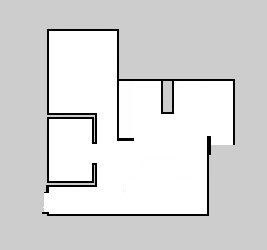
\includegraphics[width=7cm]{img/cap4/mapaestatico}
  \end{center}
  \caption{Mapa estático}
  \label{fig:mapaestatico}
\end{figure}

\subsection{Mapa de corto plazo}
El mapa de corto plazo se caracteriza por ser un mapa en el que se representa los objetos que el robot va percibiendo. Este mapa se inicializa con el valor 255, lo que indica una incertidumbre total. En el instante en el que el algoritmo de construcción del mapa comienza a iterar comenzarán a corregirse estos valores iniciales, asignando el valor 0 a las celdas que corresponden con zonas libres e incrementando desde 0 hasta 254 el valor de las celdas que se perciben como ocupadas. \pagebreak

\renewcommand{\lstlistingname}{Código}
\begin{lstlisting}[caption=Inicialización del cost\_map correspondiente al mapa de corto plazo, label={lst:initcostmap}]

  metadata = getMetadata();
  tf::TransformListener tf(ros::Duration(10));
  cells_size_x = metadata.width;
  cells_size_y = metadata.height;
  resolution = metadata.resolution;
  origin_x = metadata.origin.position.x;
  origin_y = metadata.origin.position.y;
  default_value = 255;
  scan_ready = false;
  pos_ready = false;
  cost_map.resizeMap(cells_size_x,cells_size_y, resolution, origin_x, origin_y);
  cost_map.setDefaultValue(default_value);
  cost_map.resetMap(0,0,cost_map.getSizeInCellsX(), cost_map.getSizeInCellsY());
\end{lstlisting}


El algoritmo propuesto destaca por la capacidad de no solo añadir objetos al mapa, si no ademas eliminarlos si los objetos desaparecen del lugar que ocupaban. Para ello se compara cada muestra de datos con el mapa que estamos generando y si en dicha muestra existen celdas libres que en el mapa están ocupadas se decrementa el valor de dicha celda en el mapa. La cuantía del decremento se puede modelar, consiguiendo así que el robot olvide más lentamente o más rápidamente los objetos que desaparecen del escenario.\\

\renewcommand{\lstlistingname}{Código}
\begin{lstlisting}[caption=Función que actualiza el mapa en cada iteración, label={lst:updatecostmap}]
  void
  ObstacleDetector::updateCostmap(){
    if(scan_ready && pos_ready){
      incrementCostProcedure();
      decrementCostProcedure();
    }
    pVectorList_.clear();
    pointList_.clear();
  }
\end{lstlisting}

La figura \ref{fig:initserver} fue captada al iniciar el algoritmo. Observamos que la mayor parte del mapa de corto plazo se encuentra en una posición de desconocimiento y que se han ido incluyendo en este las zonas libres, las paredes y la estantería. Los puntos morados y verdes corresponden a la representación de las muestras tomadas por el láser.

\begin{figure}[H]
  \begin{center}
    \subfigure[]{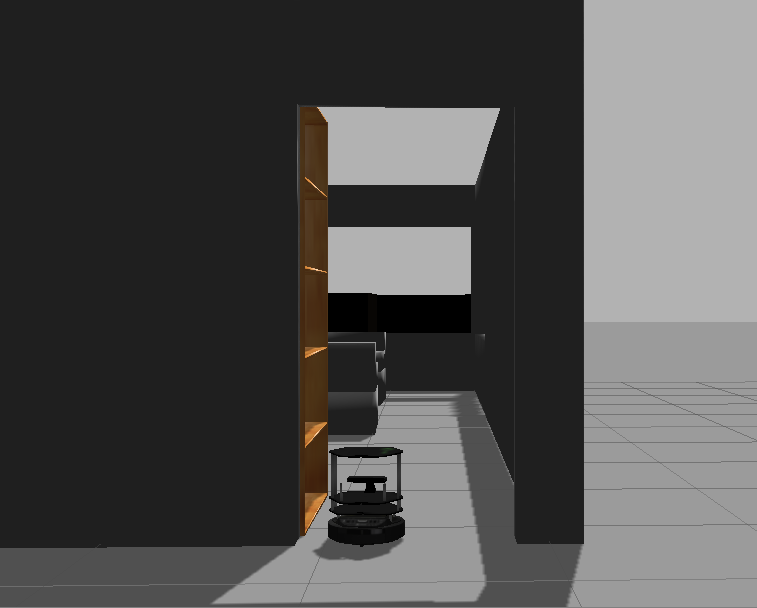
\includegraphics[width=5cm,height=5cm]{img/cap4/incrementmap}}
    \subfigure[]{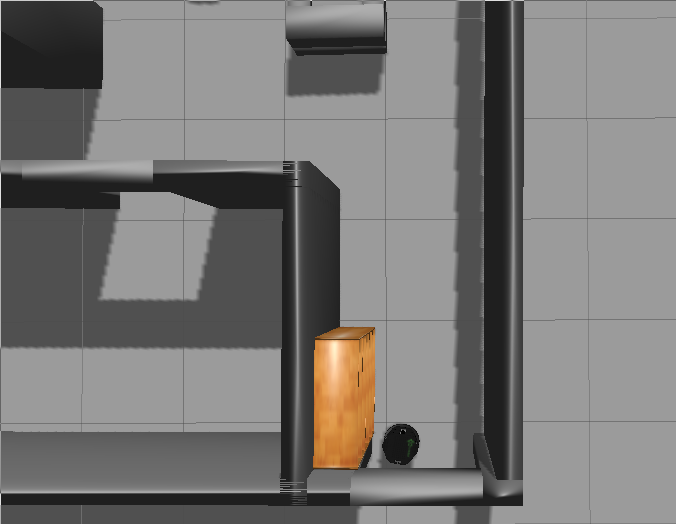
\includegraphics[width=5cm,height=5cm]{img/cap4/incrementmap2}}
    \subfigure[]{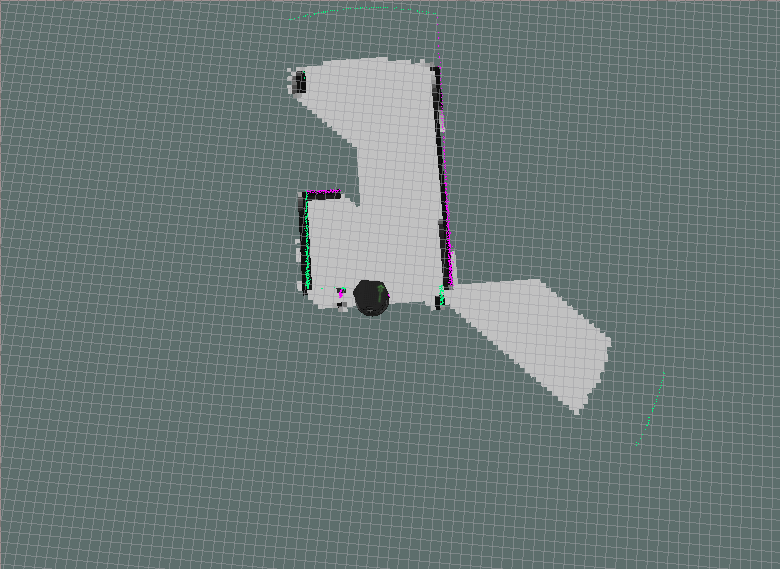
\includegraphics[width=5cm,height=5cm]{img/cap4/incrementmap-rviz}}
  \end{center}
  \caption{Visión del simulador, (a) y (b), y mapa a corto plazo (c).}
  \label{fig:initserver}
\end{figure}

Tras el inicio del algoritmo se añadió un objeto nuevo al escenario. Esto se representa en la figura \ref{fig:includeobject}. Vemos como el algoritmo añade el objeto al mapa y lo sitúa en una posición coherente respecto a la posición que ocupa el objeto en el escenario simulado.

\begin{figure} [H]
  \begin{center}
    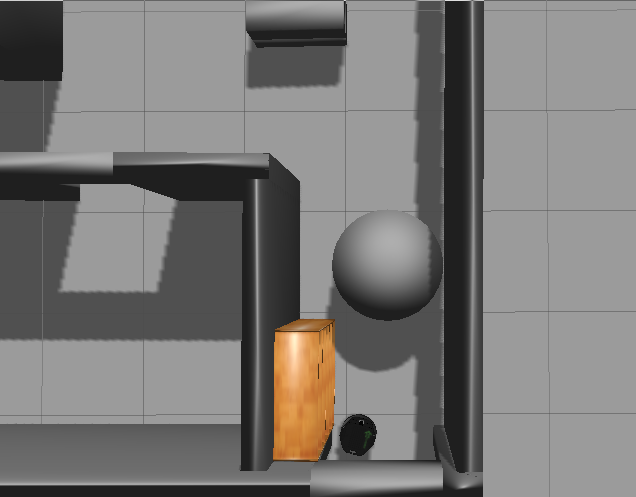
\includegraphics[width=6cm,height=5cm]{img/cap4/incrementmap-object3}
    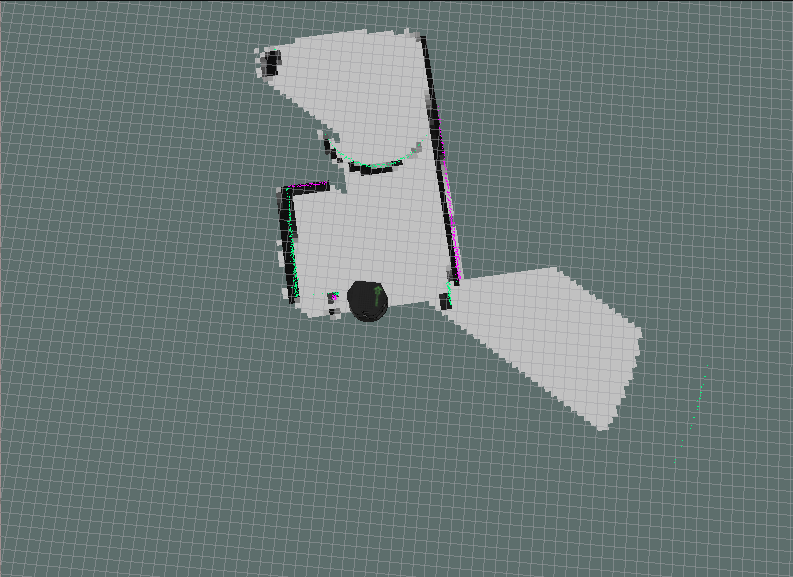
\includegraphics[width=6cm,height=5cm]{img/cap4/incrementmap-object}
  \end{center}
  \caption{Añadimos un objeto al escenario}
  \label{fig:includeobject}
\end{figure}

Una vez que el algoritmo a incluido el objeto en el mapa procedemos a eliminarlo del escenario simulado. Esto se representa en la figura  \ref{fig:deleteobject}. Vemos como el algoritmo ha comenzado a borrar el objeto, por lo que el valor de las celdas que estaban ocupadas por el objeto ahora es mucho menor.

\begin{figure}[H]
  \begin{center}
    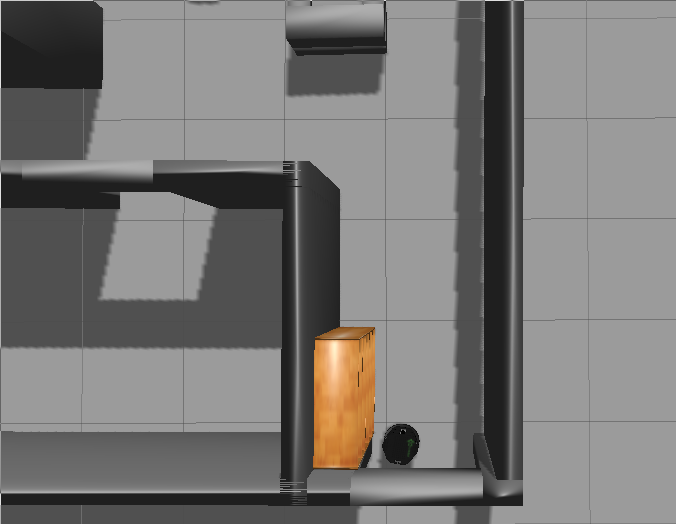
\includegraphics[width=6cm,height=5cm]{img/cap4/incrementmap2}
    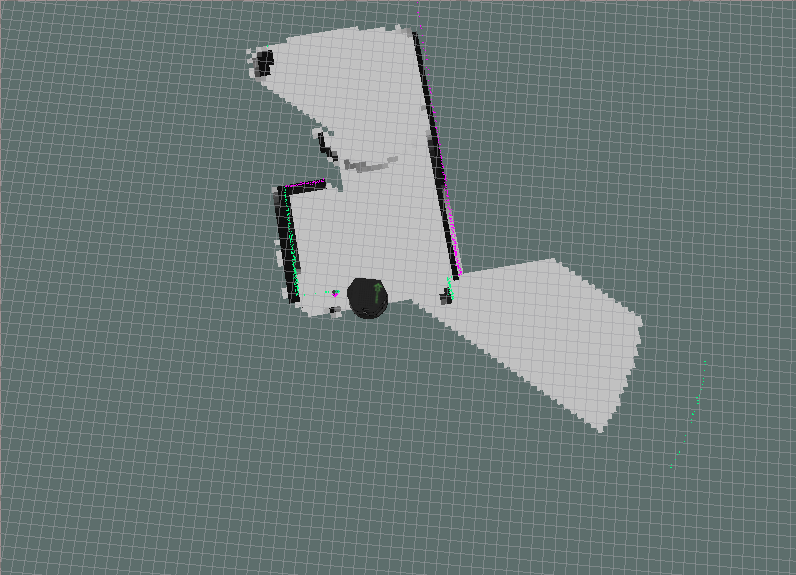
\includegraphics[width=6cm,height=5cm]{img/cap4/incrementmap-object2}
  \end{center}
  \caption{Eliminamos un objeto del escenario}
  \label{fig:deleteobject}
\end{figure}

El proceso de añadir o eliminar un objeto puede ser más o menos rápido dependiendo de los valores de las variables que modelan estas operaciones. Para el caso de nuestro algoritmo contamos un fichero con extensión yaml en el que modificamos los valores de los parámetros.
\renewcommand{\lstlistingname}{Código}
\begin{lstlisting}[caption=Fichero de configuración obstacle\_detector.yaml, label={lst:obstacledetectorconfig}]
  cost_inc: 4
  cost_dec: 1
  min_lenght: 0.23
  max_lenght: 2.5
\end{lstlisting}
Los valores asociados a cost\_inc y cost\_dec representan el incremento o decremento del valor de una celda por cada iteración del algoritmo. Los otros valores configurables representan la longitud máxima y mínima que se tiene en cuenta para cada medida que el láser nos proporciona. Las muestras obtenidas del láser que estén fuera de estos valores son ignoradas.

{Explicar como se borran los objetos? (decremento)}\\

Al final de cada iteración del algoritmo el mapa de corto plazo es publicado en un topic para que pueda ser usado por el resto de nodos que conforman el servidor de mapas dinámico. Para llevar a cabo esta operación usamos una estructura de datos proporcionada por ROS, \textit{Costmap2DPublisher}\footnote{http://docs.ros.org/indigo/api/costmap\_2d/html/classcostmap\_\_2d\_1\_1Costmap2DPublisher.html}. Este publicador publica nuestro mapa en el topic \textit{costmap\_auto}.\pagebreak
\renewcommand{\lstlistingname}{Código}
\begin{lstlisting}[caption=Step del nodo obstacle\_detector, label={lst:stepobstacledetector}]
  void
  ObstacleDetector::step(){
    updateCostmap();
    cost_map_publisher_.publishCostmap();
  }

  int
  main(int argc, char** argv)
  {
    ros::init(argc, argv, "obstacle_detector");   //Inicializa el nodo
    ObstacleDetector obs;
    ros::Rate loop_rate(5);

    while (ros::ok()){
      obs.step();
      ros::spinOnce();
      loop_rate.sleep();
    }
    return 0;
  }

\end{lstlisting}

Existe un pequeño cambio en los valores del mapa que se publica. El tipo de mensaje que se usa para publicar un costmap es \textit{nav\_msgs::OccupancyGrid}\footnote{http://docs.ros.org/indigo/api/nav\_msgs/html/msg/OccupancyGrid.html}. Este tipo de mensaje contiene, ademas de los metadatos asociados al mapa, un array de datos que representa al mapa. La principal diferencia con un costmap es que los valores en un OccupancyGrid van de 0 a 100 y -1 para las celdas desconocidas ,y no de 0 a 255 como en un costmap.

\subsection{Mapa de largo plazo}
El mapa de largo plazo se inicializa con los valores del mapa estático y se caracteriza por incluir los objetos que tienen un valor muy alto en el mapa de corto plazo, por tanto tenemos un mapa con objetos que han perdurado en el mapa a corto plazo durante un largo periodo de tiempo y que podemos considerar que nos van a influir a la hora de planificar nuestra ruta por el escenario. 
Este mapa también es dinámico, por lo que también elimina los objetos del mapa si estos desaparecen o cambian su posición.
\pagebreak 

\begin{lstlisting}[caption=Procedimiento para añadir un objeto al mapa de largo plazo, label={lst:addobjectlongmap}]
  void
  MapController::updateLongTermMap(nav_msgs::OccupancyGrid s_map){
    for(int i = 0;i<s_map.data.size();i++){
      if(s_map.data[i] > 95){
        longTerm_map.data[i] = s_map.data[i]; 
        .
        .
        .
      }
    }
  }

\end{lstlisting}

En el código mostrado en \ref{lst:addobjectlongmap} muestra el proceso de adición de un objeto al mapa de largo plazo. Para ello se recorren los valores del mapa de corto plazo y si alguno tiene un valor mayor a 95, valor que consideramos lo suficientemente alto como para que sea muy fiable que esa celda está ocupada, se incluye con ese valor al mapa.

\begin{figure}[H]
  \begin{center}
    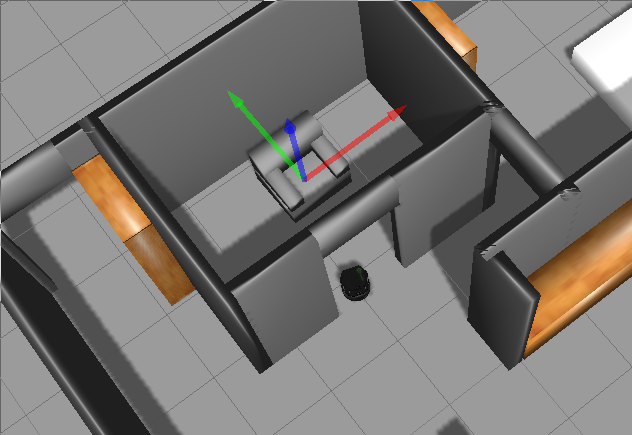
\includegraphics[width=10cm,height=6cm]{img/cap4/addingobject-gazebo}
    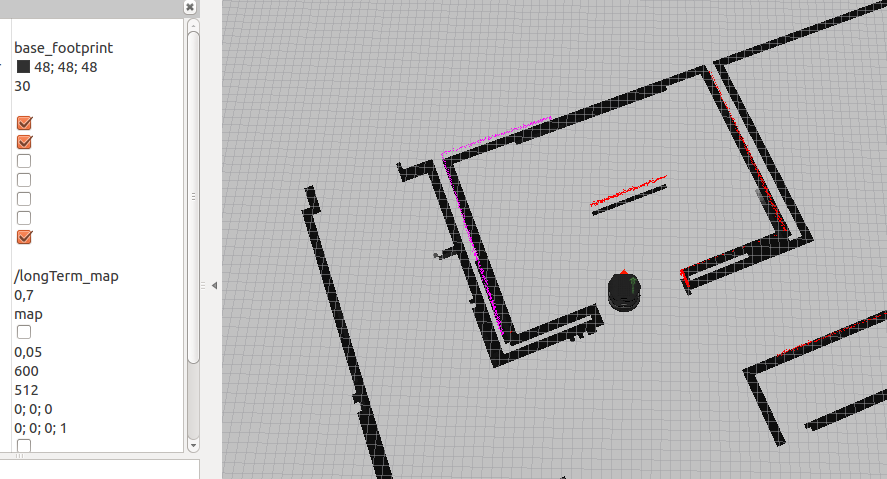
\includegraphics[width=10cm,height=5cm]{img/cap4/addingobject-longmap}
  \end{center}
  \caption{Añadimos un objeto al mapa de largo plazo}
  \label{fig:addobjectlongmap}
\end{figure}
\pagebreak


\begin{lstlisting}[caption=Procedimiento para eliminar un objeto al mapa de largo plazo, label={lst:deleteobjectlongmap}]
  void
  MapController::updateLongTermMap(nav_msgs::OccupancyGrid s_map){
    for(int i = 0;i<s_map.data.size();i++){
      .
      .
      .
      }else if(s_map.data[i] < 5 && s_map.data[i] >= 0 && longTerm_map.data[i] >= longterm_cost_dec && static_map.data[i] < 95){
        longTerm_map.data[i] = longTerm_map.data[i] - longterm_cost_dec;
      }
    }
  } 

\end{lstlisting}

En el código mostrado en \ref{lst:deleteobjectlongmap} se compara el mapa de largo plazo con el mapa de corto plazo. Si una celda en el mapa de largo plazo tiene un valor que indica que está ocupada y en el mapa de corto plazo esa misma celda tiene un valor que indica que está libre, siempre y cuando esa celda no pertenezca a una celda de una pared, se decrementa su valor en el mapa de largo plazo. La cuantía de este decremento también puede modelarse, longterm\_cost\_dec, regulando así la memoria que tenemos de los objetos que hemos añadido a este mapa.\\

\begin{figure}[H]
  \begin{center}
    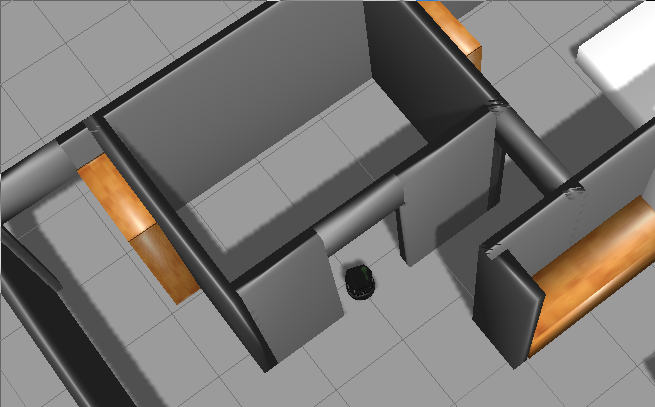
\includegraphics[width=10cm,height=5cm]{img/cap4/deletingobject-gazebo}
    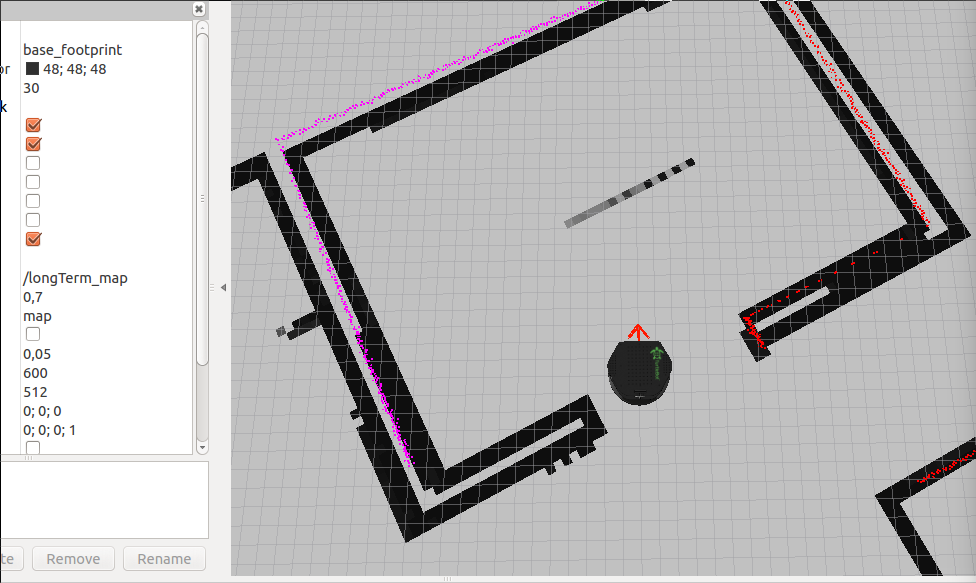
\includegraphics[width=10cm,height=5cm]{img/cap4/deletingobject-longmap}
  \end{center}
  \caption{Borramos un objeto del mapa de largo plazo}
  \label{fig:deleteobjectlongmap}
\end{figure}

Por último publicamos el mapa en el topic \textit{/longTerm\_map}.

\begin{lstlisting}[caption=Publicación del mapa de largo plazo, label={lst:longmappublish}]
longTermMap_pub   = nh_.advertise<nav_msgs::OccupancyGrid>("/longTerm_map", 5); 

void
MapController::publishAll(){
  .
  .
  .
  longTerm_map.header.stamp = ros::Time::now();
  longTermMap_pub.publish(longTerm_map);
}
\end{lstlisting}


Adicionalmente este mapa se guarda cada cierto tiempo en un fichero, usando el nodo por defecto de ROS para este fin ,\textit{map\_saver}\footnote{http://wiki.ros.org/action/fullsearch/map\_server\#map\_saver}. Así por ejemplo podemos tener un cuenta una mesa dentro del salón de una casa para una futura ejecución del algoritmo. Esto nos permitiría planificar una ruta mejor para la navegación, ya que podríamos esquivar esta mesa con facilidad y llegar a nuestro destino lo más rápido posible. Si no tuviéramos esta mesa en cuenta el algoritmo podría planificar una ruta a través de las celdas ocupadas por la mesa. Seguramente el robot no llegaría a chocar, ya que el planificador de rutas usa un pequeño mapa local para evitar estos problemas, pero es seguro que tardaría más en alcanzar su destino ya que al encontrarse frente a la mesa el robot se pararía y tendría que recalcular una nueva ruta. 



\section{Construcción del mapa final}
\label{sec:construccionmap}
El mapa final será la composición de los mapas de largo plazo, que ya incluye el mapa estático, y de corto plazo. Este mapa será usado por el nodo de la navegación y por el nodo de la localización para navegar y localizar al robot en el escenario. La composición del mapa final o mapa efectivo será el resultado de la operación de máximo entre los mapas de corto y de largo plazo, como vemos en el código del apartado \ref{lst:buildEffectivemap}. De esta manera incluiremos en el mapa final toda la información relacionada con los objetos que llevan un tiempo en la escena y también incluiremos, aunque con un menor valor, personas o cosas que acaban de entrar en las inmediaciones del robot.
\pagebreak

\begin{lstlisting}[caption=Composición del mapa final, label={lst:buildEffectivemap}]
  void
  MapController::buildEffectiveMap(nav_msgs::OccupancyGrid s_map,nav_msgs::OccupancyGrid l_map){
    for(int i = 0;i<s_map.data.size();i++){
      effective_map.data[i] = std::max(s_map.data[i],l_map.data[i]);
    }
  }
\end{lstlisting}

Tras la creación del mapa este es publicado en el topic \textit{/map}. 

\begin{lstlisting}[caption=Publicación del mapa final, label={lst:effectivemappublish}]
effectiveMap_pub = nh_.advertise<nav_msgs::OccupancyGrid>("/map", 5);

void
MapController::publishAll(){
  effective_map.header.stamp = ros::Time::now();
  effectiveMap_pub.publish(effective_map);
  .
  .
  .
}
\end{lstlisting}


Este topic es usado por defecto por las aplicaciones que necesitan un mapa como parámetro de entrada. En nuestro caso las aplicaciones que usarán nuestro mapa son el nodo de localización y el nodo de navegación, como veremos en el siguiente capitulo. 